\documentclass[prodmode]{acmlarge}


% Metadata Information
\acmVolume{2}
\acmNumber{3}
\acmArticle{1}
\articleSeq{1}
\acmYear{2010}
\acmMonth{5}

%\usepackage[super,sort&compress]{natbib}
%\usepackage[super,sort&compress]{natbib}
%\bibliographystyle{abbrvnat}
%\renewcommand{\bibnumfmt}[1]{#1}

%\usepackage{amssymb}
%\usepackage{amsmath}
%\usepackage{amsthm}
%\usepackage{color}
%\usepackage{listings}

\usepackage{url}
\usepackage{dblfloatfix}
\usepackage{fixltx2e}
\usepackage{fancyvrb}

%\renewcommand{\artnum}{}
%\renewcommand{\firstfoot}{}

% Title portion
\title{Sigma: Android Binder Services over Network}
\author{KASTURI RANGAN RAGHAVAN,~~~
Advisor: MANI SRIVASTAVA\\ University of California, Los Angeles~~~
Masters Comprehensive Project
}
%\terms{}

\begin{document}
%\pagestyle{empty}
\maketitle
%\vspace{-8mm}

\section{Introduction and Problem Definition}

It should be easy to develop distributed mobile applications. Ideally, following the idioms of a mobile platform. With a focus on Android, this paper is an attempt to generalize its runtime to support distributed communication with other Android Devices. We chose Android as it is the most popular mobile platform today, and its the core runtime is open source so is open to experimentation. The goal and constraint is take the service-oriented Android architecture and make it available over the network as a natural way for Android devices to communicate with each other.

A variety of mobile applications can be implemented via distributed communication, below is a discussion of two categories, as motivation.

\subsubsection{Social apps}
The vast majority of social networks such as Facebook and Twitter follow the client-server model for providing service. Rightly so, the amount of historical content served and the ability to browse through a global set of peoples' profiles all require a data center's vast storage and serving capability. Attempts such as Diaspora~\cite{Diaspora} to decentralize social networks are not successful, but prove that the distributed model is possible for complex applications.

However, a niche of social services can be implemented via purely distributed communication between participating devices. Though, a central server may be used occasionally for authenticating and establishing a network among participants. Instant messaging is a good example. It is the case that voice and video chat use a peer-to-peer model of communication.

Location sharing apps give users a glimpse into a small set of friends' location and activities. Apps like Apple's FindMyFriends~\cite{FindMyFriends} or Glympse~\cite{Glympse} on the Google Play Store are good examples. Although it is unknown whether such proprietary apps use a peer-to-peer or client-server approach (probably the latter), from their functionality alone it seems feasible to implement the service with the former. That is because the basic usefulness is garnered from the streaming of real-time data, so necessarily all active participants must be reachable over the network. There is no need for serving historical data, and the group of participants typically stable and small.

There are also a class of services characterized by the sharing of ephemeral data. The most popular such service is Snapchat--a photo messaging app where recipients see the photos shared with them for a brief period (1 to 10 seconds) and then it disappears~\cite{Snapchat}. The nature of the service is something that affords participants some privacy, knowing that recipients can only briefly glimpse at shared pictures.

"Snapchat is a super interesting privacy phenomenon because it creates a new kind of space to communicate, which makes it so that things that people previously would not have been able to share, you now feel like you have place to do so," says Mark Zuckerberg--CEO of Facebook. "That’s really important, and that’s a big kind of innovation that we’re going to keep pushing on and keep trying to do more on, and I think a lot of other companies will, too."~\cite{Zuckerberg}

However, Snapchat as it is implemented today follows a client-server model. Shared pictures are first pushed to the cloud and then pushed to recipients~\cite{SnapchatHack}. This much is known, because a security breach at Snapchat established that shared pictures (thought to be privately shared and ephemeral) are stored by Snapchat servers long after they have been viewed by recipients. For such a privacy-promoting service a peer-to-peer model looks to be an even better fit, as pictures do not need to transit (or stored) in the cloud for any period of time. It seems that the issue of privacy motivates the push towards the peer-to-peer modeling of mobile services.

\subsubsection{Internet of Things}
Another source of demand for a distributed communication framework is from the Internet of Things (IoT). In this new internet, devices have a need to send control commands or to poll for sensor readings from another device. It is likely that Android will be the primary platform used inside smart gadgets consisting the IoT. Already consumer products like the \$30 Chromecast--a barebones Android device that plugs into the HDMI port on TVs--is capable of receiving video streams and display from other Android devices over LAN~\cite{chromecast}. Chromecast communicates with other Android devices and Chrome browsers using webrtc, an emerging W3C standard P2P technology~\cite{ChromecastWebrtc}. Future internet-enabled home appliances will probably use Android~\cite{AndroidEverywhere} in some form--the recent Google acquisition of Nest~\cite{GoogleNest} who formerly made smart home thermostats lends some support to that possibility. We see already frameworks like the Eclipse M2M  stack for distributed communication between embedded devices~\cite{eclipse_m2m}.

\subsection{Related work}
Related work in this field include projects like Interdroid~\cite{Interdroid} whose goals are close to this project: which is to create a platform for distributed applications. Or there are the basic implementations of peer-to-peer networking like that found in webrtc. However these technologies all exist as add-on java packages and/or native libraries. Related to privacy, there is πBox~\cite{piBox}: a platform for privacy-preserving apps, achieving a sandbox that spans across devices, providing secure channels (a specific non-Android API) for enabling app functionality.

\subsection{Goals and Constraints}
The inspiration for this paper is in part from the well-known X windows system. It is a server that provides display and input-devices operations. Applications follow a simple protocol (X11) to create and coordinate GUI interactions, and the server sends over input-device actions. It is fully message-based protocol, and is specifically designed to allow for messages to be tunnelled network connections~\cite{X11}. This allows applications running on one machine to be displayed and controlled via a remote X11 server. Thus, anyone with an interactive terminal can interact with GUI applications.

Similarly, Android services are provided with an underlying message-based protocol--as we will see in detail. Assuming these messages can be tunneled through a network connection, it should be possible to have Android apps access remote Android services. And in turn, for remote Android services to callback local apps or make use of local services--effectively creating a distributed communication platform.

None of the related projects, to the best of our knowledge, allow the creation of distributed apps while following the very same service-oriented architecture provided by Android. It should be easy to develop distributed mobile applications following idiomatic service paradigms in Android. This paper takes a step towards the goal by observing that the Android framework closely follows a service-oriented architecture, enabled by a service-oriented interprocess- communication (IPC) mechanism known as Binder. It is my hypothesis that this architecture will generalize well to become a framework for distributed communication between Android devices. Binder is the primary encouraged mechanism to  provide services on Android, and it enjoys great programmer support for implementing RPCs by way of SDK tools.

This paper presents Sigma, an implementation of a distributed communication framework on Android that builds upon the Binder framework. The rest of the paper is organized as follows. First is an overview of Binder from its kernel module implementation to its OO abstractions in the Android Runtime. Next is an overview of a subset of Android system services which can be made available over the network. Then the design and implementation detail of Sigma, presenting an overall design idea followed by a systematic implementation detail of each piece. To evaluate the design and test performance we present some example applications. (1) Parts of Sigma itself are available as a remotable binder service (2) A set of test cases that evaluate the additional costs (of latency and CPU time) of Sigma on implemented locally, over HTTP and over XMPP. (3) A Snapchat-clone implemented in Binder. Finally, a discussion about limitations and drawbacks, and next steps.

\section{The Android Binder Framework}
The Binder framework is Android's primary interprocess-communication (IPC) mechanism, and it is used widely within the Android Runtime. System services are provided through binder.
A binder allows a process to present an specific interface as a service which may be called by other threads or processes. A binder call is essentially a remote procedure call (RPC) with communication between linux processes achieved using ioctl calls on a file descriptor. The binder at its most basic level is a kernel module. As such binder maintains isolation between processes, maintaining modularity and privilege separation as implemented by the linux kernel~\cite{OpenBinder}.

\subsection{Kernel Module}
The binder kernel module (BKM) provides the facility to register a default binder service known as the system context manager. It is then job of the context manager to manage binder objects in the operating system. This context manager can be accessed by arbitrary processes via a call to the BKM. In Android the context manager presents an IServiceManager interface. The ServiceManager starts at boot-up as the root system process, and is registered as the context manager with BKM. It manages a directory system services, and as system services publish themselves to the directory via binder RPC.

Using the lowest-level API for binder, here are the sequence of commands to create and publish a binder service. The provided service is implemented via a handler function, not shown here. The arguments to binder\_call are described in the appendix.

\begin{Verbatim}[samepage=true]
binder_state* binder_service = binder_open();
binder_state* publish_txn = binder_open();

// RPC to the ServiceManager to publish the
// service, details of arguments to binder_call
// are described in the appendix.
binder_call(publish_txn, msg, reply, (void*)0,
            SVC_MGR_ADD_SERVICE);

// loop indefinitely. Incoming transactions
// will invoke the handler.
binder_loop(binder_service,
            (void*)service_handler);
\end{Verbatim}

Note that msg and reply are binder\_io data structures that contain the data to be passed into or returned, respectively, from binder\_call. The RPC interface is defined by purely by convention. The binder\_call here to publish a service has a msg that contains data encoded to a byte array. This is shown below in pseudo-code.

\begin{Verbatim}[samepage=true]
msg = {
  /* string name of the remote interface */,
  /* string name of service being published */,
  /* flat_binder_object struct with pointer
     to binder_service */
}
\end{Verbatim}

Another process can retrieve a reference to the just-published service via RPC to ServiceManager, querying for it by name. The return value (the reply) will contain a flat\_binder\_object struct with a reference to the service. RPCs can then be made with the reference passed in as target.

\begin{figure*}
\centering
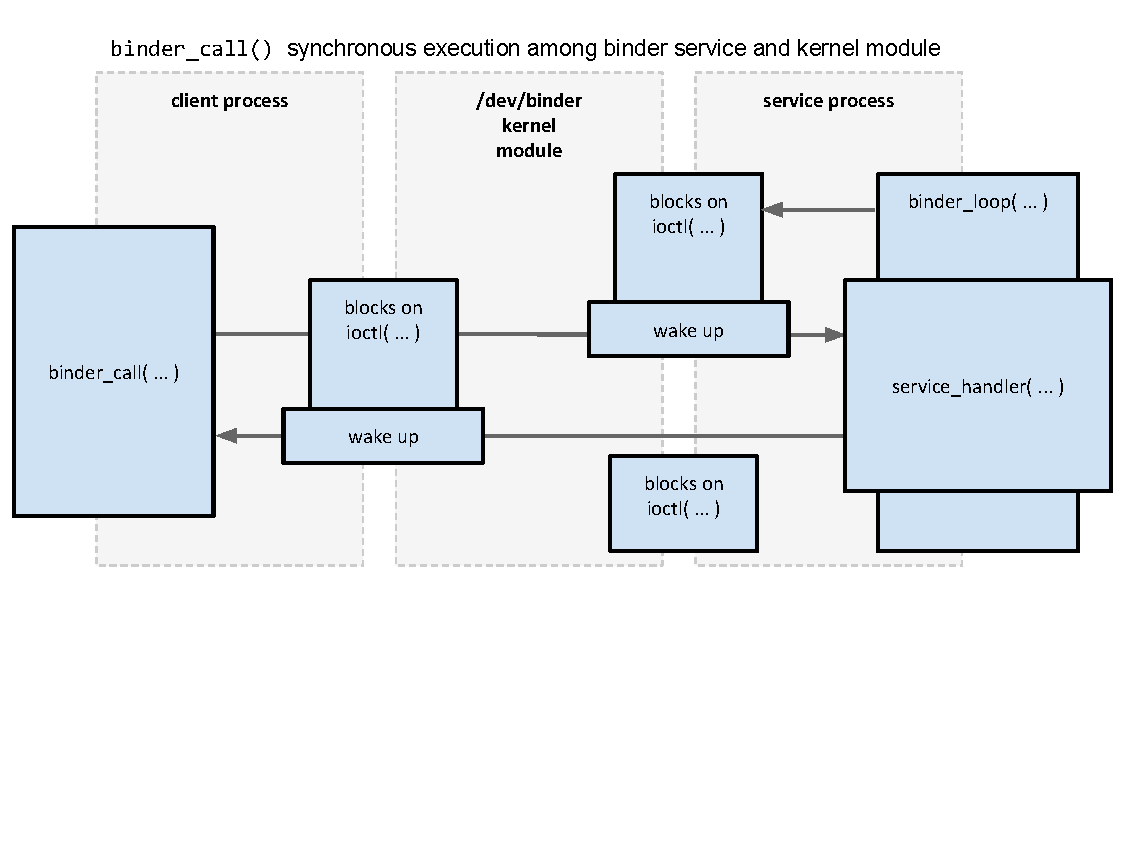
\includegraphics[width=0.75\textwidth]{drawings/binder_call.pdf}
\end{figure*}

\subsubsection{Writing objects into binder\_io}
A crucial feature of binder is the ability to write binder objects and file descriptors for RPCs. This way, a process can obtain a handle to a remote object like a remote binder service as a callback object. Primitive types are written directly, whereas object and file descriptors are written as flat\_binder\_object structs. The 'binder\_io.offsets' supplied as part of a binder transaction contains offsets into the data where these structures occur. The Binder driver takes care of rewriting the structure type and data as it moves between processes~\cite{BinderSourceComment}.

This level of overview of BKM is sufficient in detail for the scope of this paper. Documentation on internals of binder is sparse. The following references~\cite{BinderLinuxFoundation,BinderMastersThesis} provide a useful resource, but the real reference is deferred to its implementation in Android.

\subsection{Binder within the Android Runtime}
The Android Runtime has several layers of abstractions built on top of the basic BKM. All these layers eventually result in calls either to the lowest-level C API which we have just covered or directly operate on the kernel driver. The main difference is that the C++ and Java APIs are object-oriented, defining an IBinder interface which binder services implement. transact(...) is the method to perform generic operations to implement RPC. It very much resembles the low-level C API's binder\_call(...) function. The object-oriented (OO) implementation also encapsulates binder\_io structures as Parcel objects.

\begin{Verbatim}[samepage=true]
interface IBinder {
  /* Get the canonical name of the interface
   supported by this binder. */
  String getInterfaceDescriptor();
  boolean pingBinder();
  boolean isBinderAlive();
  IInterface queryLocalInterface(
      String descriptor);
  boolean transact(
      int code, Parcel data,
      Parcel reply, int flags);
  void linkToDeath(
      DeathRecipient recipient, int flags);
  boolean unlinkToDeath(
      DeathRecipient recipient, int flags);
}
\end{Verbatim}

The OO Binder follows the Proxy Pattern~\cite{ProxyPattern}. BBinder is a class that is instantiated as the real implementation of the service. It calls the equivalent of binder\_loop and accepts transaction requests. Then there is BpBinder which is a proxy class that is isntantiated with the a handle to an active BBinder service. Analogously, there is a Java implementation that has a mirror IBinder java interface~\ref{code:IBinder} with a Binder and BinderProxy which wrap BBinder and BpBinder native objects, respectively, via JNI.

An invokation of BpBinder.transact() simply invokes a binder\_call to its remote handle, and via binder invokes the BBinder.transact() method to be invoked. A service interface on top of this basic mechanism is implemented by extending the two classes and following a convention. For instance, a FooBarService is implemented by associating each method with a code.

\begin{Verbatim}[samepage=true]
class BpFooBarService : public BpBinder {
  void foo(int a, int b) {
    /* ... */ transact(1, encoded_args, ...);
  }
  void bar(string c) {
    /* ... */ transact(2, encoded_args, ...);
  }
  /* transact() calls remote binder, waits,
     and returns reply. */
}
class BnFooBarService : public BnBinder {
  void foo(int a, int b) {
    /* Do something useful */
  }
  void bar(string c) {
    /* Another useful fucntion */
  }
  void transact(code, msg, reply, flags) {
    switch(code) {
      case 1: /* decode args... */ foo(args);
             break;
      case 2: /* decode args... */ bar(args);
             break;
}}}
\end{Verbatim}


%\begin{figure}[h!]
%\centering
%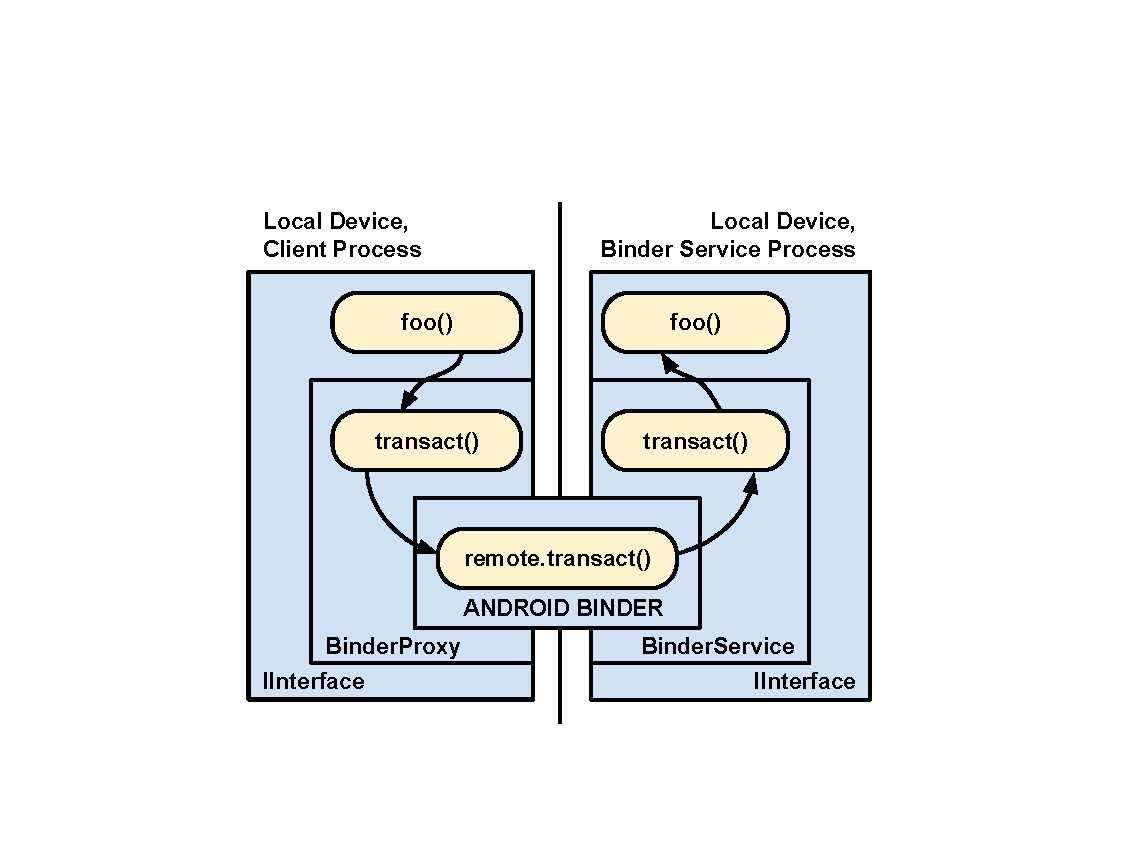
\includegraphics[width=0.8\columnwidth]{drawings/proxy_pattern.pdf}
%\end{figure}

The creation of binder RPC involves boilerplate code. To make this more convenient, the Android SDK defines a domain-specific language named AIDL to specify interfaces for binder services in a language similar that that for specifying Java interfaces. The AIDL compiler generate Stub and Proxy classses that implement the specified interface and contain internal fields to Binder and BinderProxy objects, respectively. A developer simply extends the Stub object, providing an implementation for each specified method (like foo() and bar() above). The generated classes do all the necessary work to marshall and unmarshall arguments as Parcels and invoke the appropriate method on the actual service object.

\begin{Verbatim}[samepage=true]
interface FooBarService {
  void foo(int a, int b);
  void bar(String c);
}
\end{Verbatim}

A binder object implementing a specified service can be created simply by extending the Stub class, providing an implementation for specified methods.
\begin{Verbatim}[samepage=true]
IBinder localBinder = new FooBarService.Stub() {
  void foo(...) { ... }
  void bar(...) { ... }
};
\end{Verbatim}

\subsection{Accessing Binder Services}
The Android Runtime provides ways to communicate binder objects to other processes. For instance, Android apps can declare a Service component that other components like GUI Activity components can bind to.

\begin{Verbatim}[samepage=true]
class FooBarAndroidService extends Service {
  public void onBind() {
    return new FooBarService.Stub() { ... }
  }
}

class FooBarClient extends Activity {
  public void onStart() {
    bindService(/* name of the service */,
                /* callback on connected */ this);
  }

  public void onServiceConnected(
    Context context, IBinder binder) {
    // The binder we get is a BinderProxy.
    // Call a method via RPC--transits through
    // the binder kernel module.
    FooBarService.asInterface(binder).foo(1, 3);
  }
}
\end{Verbatim}

As we see above, retrieving a non-system service is just a simple asynchronous operation from the perspective of the app developer. However, there are a few core services of the Android Runtime that come into play to make it happen.

\begin{figure*}
\centering
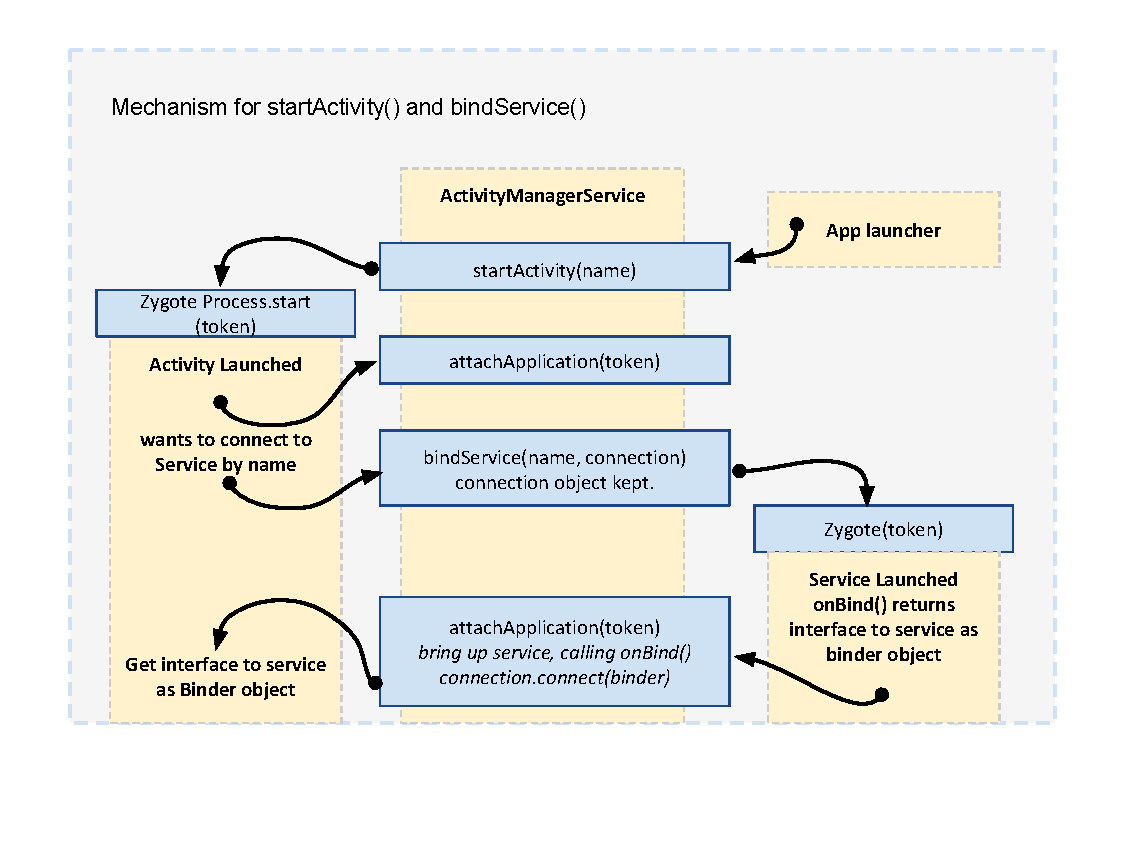
\includegraphics[width=0.75\textwidth]{drawings/bindService.pdf}
\end{figure*}

bindService(...) is invoked with a callback binder object--the ServiceConnection. Once the requested service is up, the ServiceConnection callback is invoked asynchronously with the requested binder service as an IBinder object. The ActivityManager works together with other essential system services to bring up and connect to the specified service component. The PackageManager, which tracks all installed components on the system, validates that the requested service component exists and checks that the caller has permissions to connect to it. If the requested service resides in a separate java package, a low-level component known as Zygote brings up the service as a separate process. When the service is up, it attaches to the ActivityManager via RPC. Afterwards, ActivityManager retrieves the binder service provided by the service component as an IBinder object, and passes it on the caller by invoking the ServiceConnection callback. There are quite a few RPCs involved in this procedure!

\subsubsection{Accessing Android System Services}
bindService(...) cannot be used for everything. For instance, in the course of binding to a service, the ActivityManager brings up the service first and waits for it to attach. The service cannot use bindService() to get a reference to the ActivityManager, as that is a circular dependence. Instead core system services like ActivityManager are all available through the ServiceManager--the binder kernel module's default context manager. It is straightforward to obtain a reference to the ServiceManager from any process or thread (i.e. make binder\_call with target=(void*)0). So it follows that it is always possible to retrieve IBinder references to any currently active service published to the ServiceManager.

ServiceManager also has an OO Binder implementation. Its interface is provided in the Appendix. The manual binder\_call() we had done to publish a service in the first section discussing the BKM is a less convenient alternate.

\section{Does it make sense to access System Services over the Network?}
Before going into the design and implementation of Sigma, it is useful to understand first what all system services that are offered via binder. This will serve as motivation to figure which feature of binder we will have to support in Sigma. In particular, we want to answer: which services are useful for remote devices to access? And which cannot be accessed (or don't make any sense to provide access to)?  To start, it is reasonable to expose ServiceManager since it is an entry-point into all other system services. There are dozens of system services, four are covered here.

\subsection{LocationManager: location updates via binder callback and PendingIntent}
It is most natural to expose system services that are standalone and isolated in a sense. A good example is the LocationManager which "allows applications to obtain periodic updates of the device's geographical location, or to fire an application-specific Intent when the device enters the proximity of a given geographical location.~\cite{LocationManagerDocs}" The location manager operates as a standalone source of location updates. Here are 2 methods of the LocationManager that we look into further.
\begin{Verbatim}[samepage=true]
interface ILocationManager {
  void requestLocationUpdates(
      in LocationRequest request,
      in ILocationListener listener,
      in PendingIntent intent,
      String packageName);
  void removeUpdates(
      in ILocationListener listener,
      in PendingIntent intent,
      String packageName);
  // ... among other methods
}
\end{Verbatim}

\begin{Verbatim}[samepage=true]
oneway interface ILocationListener {
    void onLocationChanged(in Location location);
    // ... among other callback methods
}
\end{Verbatim}

The main requestLocationUpdates() method requires the client to provide either a ILocationListener binder callback or PendingIntent callback. If the former callback is initialized locally and passed in as a binder argument. Then the LocationManager holds a weak reference to it and and invokes the .onLocationChanged() callback periodically with location updates. The provided binder object must remain active for it to receive callbacks.

The latter PendingIntent callback is also works internally through binder. However the mechanism is provided by the Android Runtime. A PendingIntent is owned by the Android Runtime, and the caller first obtains a reference to it from the central ActivityManagerService. A PendingIntent is constructed with the address of a recipient (callback) android component to which future messages are delivered. Working as a callback mechanism, the PendingIntent is usually initialized with the caller's own component address. When provided as argument to the requestLocationUpdates() method, the LocationManager later can invoke the PendingIntent.send() RPC with location updates as contained data. This RPC goes to the Android Runtime (the owner of the PendingIntent), which then via another RPC routes the message to the recipient component. Though the PendingIntent mechanism is inherently more complex, the an advantage is that the Android Runtime takes case to brings up the recipient component in case it is not already up. This way an app can register a PendingIntent callback and not have the burden of being active to receive callbacks.

\begin{Verbatim}[samepage=true]
interface IIntentSender {
  int send(
    /* The message */
    int code, in Intent intent,
    /* Address of recipient */
    String resolvedType,
    /* Send finished callback */
    IIntentReceiver finishedReceiver,
    ...);
}
\end{Verbatim}

\begin{Verbatim}[samepage=true]
oneway interface IIntentReceiver {
  void performReceive(
      in Intent intent, int resultCode,
      ...);
}
\end{Verbatim}

PendingIntent.send() is implemented in non-blocking fashion. Hidden from view, the PendingIntent is constructed with reference to a IIntentSender binder service object which is owned by (and runs within) the ActivityManager. An additional IIntentReceiver callback can be passed in with each invokation of .send() to be notified once the send operation is complete. The LocationManager uses this send and together with a finishedReceiver callback to hold what's known as a WakeLock--an Android Runtime feature used to prevent the device from entering sleep mode. Without the WakeLock, messages would be stuck in-flight and delivered only when the device wakes up from sleep.

Both direct binder object callbacks and PendingIntent callbacks should be supported by Sigma. The latter type can allow for the design of "push" services over the network where the client can register a PendingIntent with a remote service, and subsequently receive messages from it without the local app having to be active all the time. Of course, the Sigma network component in charge of receiving remote data should be active for this to work.

\subsection{SensorManager: sensor events via unix domain sockets}
The SensorManager another good candidate service to expose as a service to other devices as it is a standalone source of sensor data streams. Recently, sensors services have evolved into contextual inferences to provide the user's activity state--e.g. categories like walking or driving.

SensorManager has a binder interface implemented directly in C++ with of JNI wrappings for providing access via the Java runtime. Unfortunately, much of the JNI wrapping is hardcoded to fetch the local binder service from the local ServiceManager. So to access a remote SensorManager, we had to modify the SensorManager code in Android to allow for external binder services.

Also, SensorEvents are sent via a BitTube--an OO abstraction on top of unix domain sockets. So this is a system service that uses binder to setup a socket connection between two processes, then the subsequent communication of sensor events happens over the socket. If we are to expose SensorManager over the network, we need to the ability to send file descriptors (and importantly: IO events to those file descriptors) over the network as well.

\begin{Verbatim}[samepage=true]
class ISensorServer : public IInterface {
public:
    Vector<Sensor> getSensorList() = 0;
    sp<ISensorEventConnection>
      createSensorEventConnection()
    // ... among other methods
};
\end{Verbatim}

\begin{Verbatim}[samepage=true]
class ISensorEventConnection : public IInterface {
public:
    sp<BitTube> getSensorChannel()
    status_t enableDisable(int handle, bool enabled)
    status_t setEventRate(int handle, nsecs_t ns)
};
\end{Verbatim}

\subsection{AlarmManager: not very useful over the network}
There are some services which don't make too much sense to expose. For instance, the AlarmManager is "intended for cases where you want to have your application code run at a specific time, even if your application is not currently running." There is no need to access a remote device's alarm manager, as an application can simply make use of its own AlarmManager for registering scheduled execution. However, although there is no immediate utility to it, there is nothing technically preventing the exposure of a device's AlarmManager has a clean interface that does not require any low-level details of the client app.

\subsection{ActivityManager: difficult to expose over network without extensive refactoring}
Services that are not standalone or are coupled to the local context of Android applications are difficult to directly expose over the network. This is because the operation of such services depends on records that are local to the device. For instance, ActivityManager is a crucial system service that is charge managing all live components running on the Android device. It provides useful operations such as bindService()  However, it is not so straightforward to invoke bindService() on a remote reference to ActivityManager depends on some information about the caller process which is only available to the local.

\subsection{A caveat with Android Permissions}
A complication, particularly when dealing with system services, is that many of them require permission to access. That is, local apps declare permission to use a service, and the PackageManager grants such permission. It is not trivial to extend the Android permissions system to allow for remote binder objects. A thorough treatment of the permissions framework and its support by Sigma is a left for future work. A brief discussion on the issue is found at the end of the paper.

\section{Sigma: Design and Implementation}
\begin{figure*}
\centering
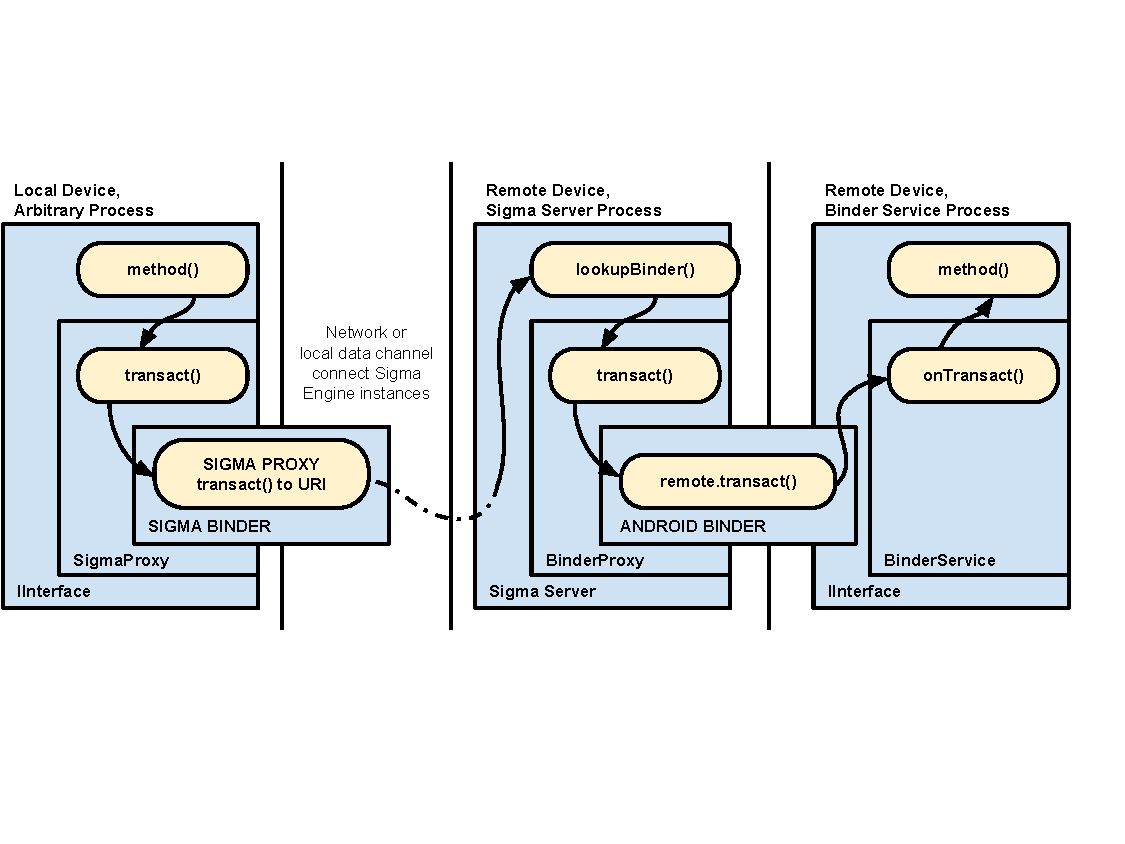
\includegraphics[width=0.8\textwidth]{drawings/sigma_proxy_pattern.pdf}
\end{figure*}
Tthe goal of Sigma is to essentially to follow the Proxy Pattern of binder services one hop out--tunneling binder transactions over the network. The design of Sigma should minimally modify the Android Runtime, while supporting both native and Java-based binder services. And, perhaps most important: Sigma should support binder's powerful feature to allow the passing of binder objects and file descriptors as arguments in a remote RPC call. This last issue will be addressed in the second-part of this section.

\subsection{Sigma as another Proxy}

Consider a network consisting of two Android devices, and that there is a pre-established data channel between them. Each device runs a Sigma Engine instance which has server-like and client-like functions. Its function viewed as a server is to associate a URI to local binder services, and subsequently accept binder transactions requests made to a URI--performing the binder transaction on the associated binder locally. Its core function as a client is to allow the retrieval of remote binder objects (retrieved as a URI) and implement the Proxy Pattern, passing on the Proxy to locally as an IBinder object. Subsequent binder transactions invoked on the proxy forward the transaction over the network to the associated URI.

Binder services are often implemented in Java with AIDL-specified interfaces. But not always. Binder services can also be hand-made (in c, c++, or java) following any arbitrary convention for doing RPC. A binder service simply has to use the BKM in some way to qualify as one. Fortunately, all Android binder services follow the IBinder interface. So the goal of Sigma is to proxy all methods of the IBinder interface. Also, fortunately, the Java and C++ versions of IBinder specify identical interfaces that are compatible with one another. In fact the Java implementation is really a JNI-based wrapper of the C++ version. So any all-native services can be first proxied into a Java BinderProxy.

Since Sigma is a network proxy, we need to have a networking stack. It makes most sense to implement this part at the Java level--using the features of the Java Android Runtime (and convenience of the SDK) to full benefit. Networking libraries are readily available for Android as pure Java libraries. Sigma is implemented as a Java-based Android application that is packaged and installed to the device as any other thirdy-party application.

\subsection{Prerequisite modifications to the Android Runtime}
There are a few obstacles to a pure Java implementation and distribution of Sigma as a simple third-party app. The default implementation of Java Binder and BinderProxy in the Android runtime does not expose native handles to BBinder and BpBinder. And there is no method exposed to create Java binder objects from native handles. So if we are to implement Sigma in pure Java running on the default Android runtime as any other app, we have no hope of creating proxy interfaces to native binder services. An example of such a service is the SensorService.

The way out is to add some methods to the Android Runtime. The following are signatures of added methods that do the job of converting from native binder to Java binder and vica-versa.

\begin{Verbatim}[samepage=true]
class BinderInternal {
  // ...
  native IBinder binderForNativeHandle(int handle);
  native int nativeHandleForBinder(IBinder binder);
}
\end{Verbatim}

A larger issue comes up when dealing with object and file descriptor arguments to RPCs. We need to specially these objects by creating proxy objects that are available over the network--the details of which we will leave for the next section. The Java and C++ OO Binder objects invoke .transact() with Parcel objects which encapsulate the underlying binder\_io data structures actually used by the kernel module. Unfortunately, the implementation of Parcel hides the underlying data structure. It does not provide access to the offsets array which contains the information about the locations where binder objects and file descriptors are written into the data array. This means we have no hope of creating proxy objects since we cannot know where they are, and so cannot read them out of the Parcel properly.
Again, the way out is to modify the Android Runtime. This time we add methods to the implementation of Parcel. Here are the method signatures of the added methods:
\begin{Verbatim}[samepage=true]
class Parcel {
  public static byte[] marshall();
  public static void unmarshall(
      byte[] data, int offest, int length);


  public static int[] getObjectPositions();
}
\end{Verbatim}

marshall() and unmarshall() are already in the default Parcel implementation, but it throws an exception when marshalling a byte array containing objects. We have fixed it to not care. Then the getObjectPositions() method fets the offsets of objects in the marshalled byte array, each of which can be read via
\begin{Verbatim}[samepage=true]
parcel.setDataPosition(offset);
IBinder binder = parcel.readStrongBinder();
\end{Verbatim}

\subsection{The Sigma Engine Protocol}
Having established that all the necessary pieces are accessible from the modified Java Android Runtime, we will now detail the design and implementation of the Sigma Engine which is a seen as protocol for retrieving binder objects as URIs and performing binder transactions on it.

Assuming we have established a data channel between two devices, we first choses a structured format for communication over the channel. There is a lightweight implementation of Google's protobuf language for serialized objects called Wire~\cite{Wire,IntroWire}. It is a open source library created specifically for Android by the Mobile app company Square. The protocol between Sigma Engines is modeled via transactions, the exchange of as Wire messages. Each transaction is composed of SRequest followed by SResponse. Pseudo-code of the protobuf implementing the generic transaction follows below:

\begin{figure}[h!]
\centering
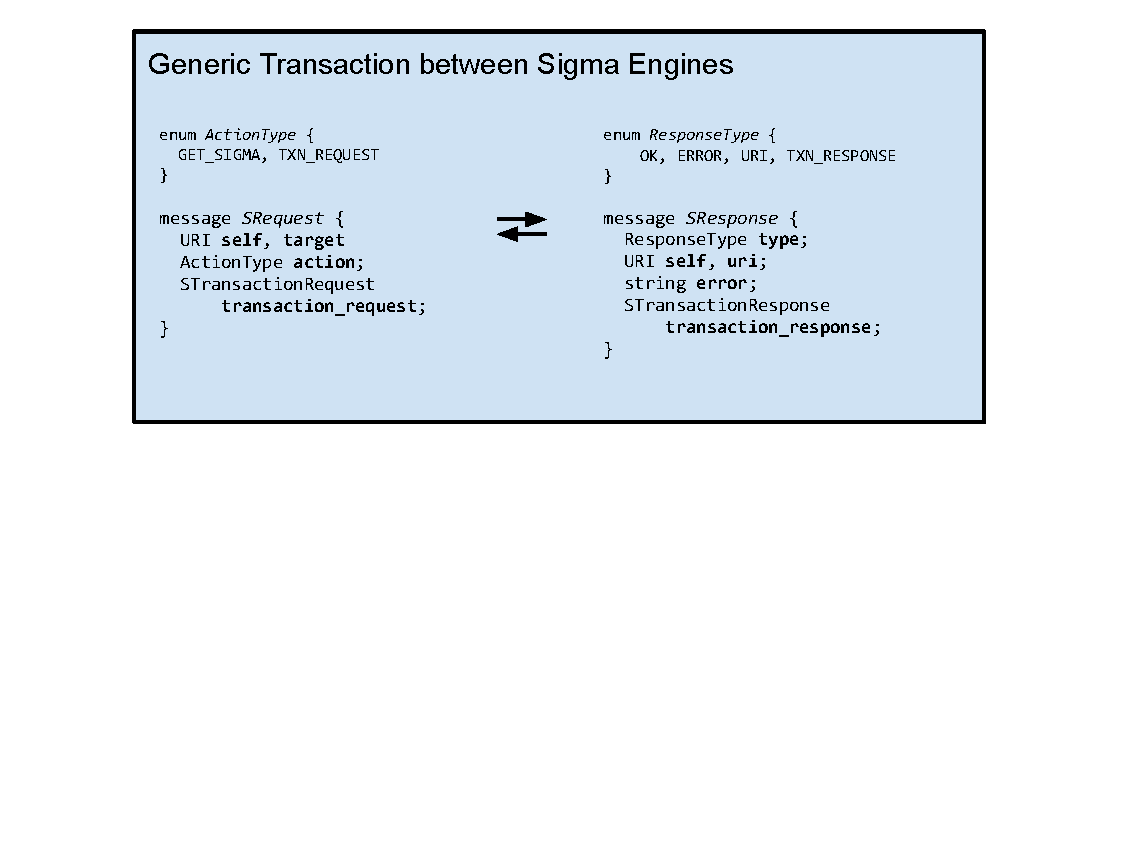
\includegraphics[width=\columnwidth]{drawings/WireTransaction.pdf}
\end{figure}

The URI is a Wire message that contains the network address of a Sigma Engine, along with any id of a contained remote object, information about the protocol, details to reach the host (e.g. host and port in the case of the HTTP protocol), and additional details about the object.

\begin{figure}[h!]
\centering
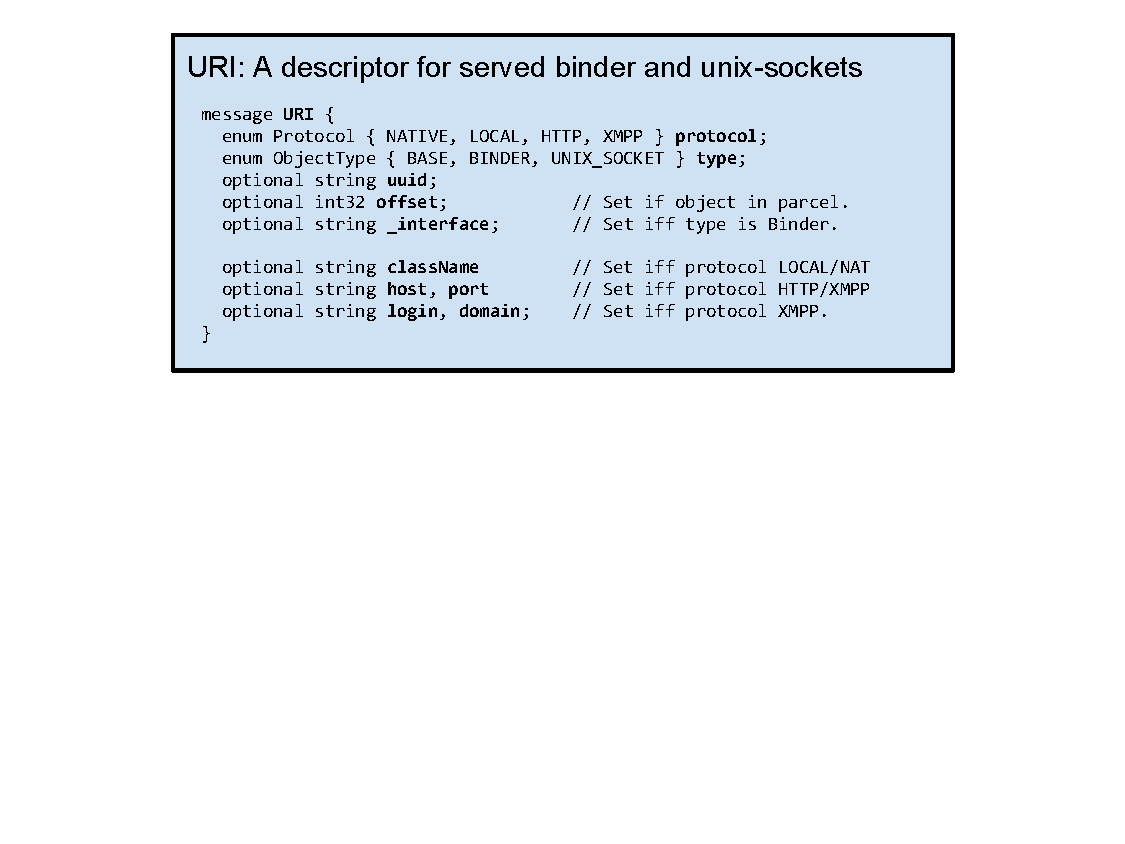
\includegraphics[width=\columnwidth]{drawings/WireURI.pdf}
\end{figure}

A proxy binder calls a remote binder's transact() method by sending the appropriate SRequest to the remote Sigma Engine. After the transaction, the remote-end sends back an appropriate SResponse. The transaction request and response both contain parcels encoded as SParcel, where the data array is first Base64-encoded to a string. And objects are specially treated--converted into URIs themselves before being sent over the network.

\begin{figure}[h!]
\centering
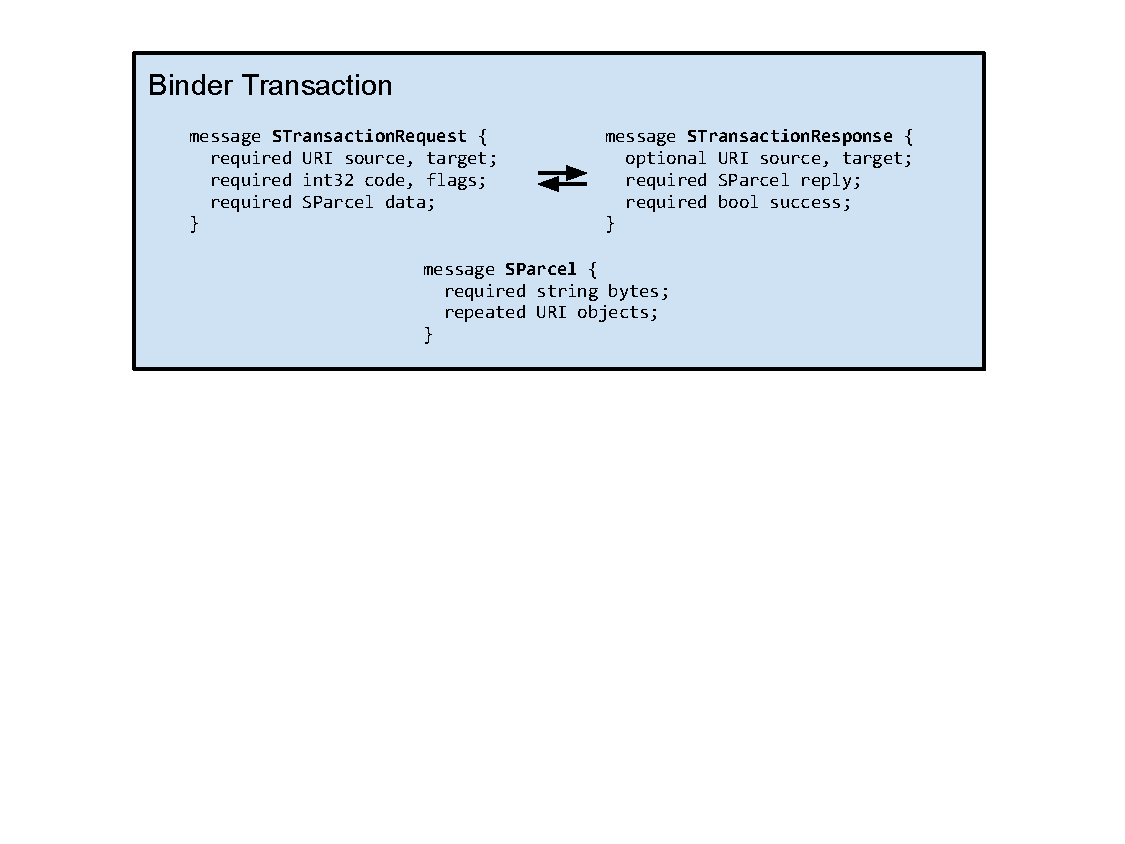
\includegraphics[width=\columnwidth]{drawings/WireBinderTransaction.pdf}
\end{figure}


\subsection{Dealing with parcels that contain binder objects}

Not everything can be copied by value when marshalling and unmarshalling Parcel objects. Binder objects are also part of the data array, and the binder\_io structure has an array offsets where each object is encoded as a flat struct.

The way we manage this is to serve each contained binder object the device's local Sigma Engine, and pass on the URI of the served object in the SParcel. On the other end, each received binder object is really received as a URI (to the corresponding remote binder object). The client creates a new SigmaProxy for each URI, writing the SigmaProxy as the binder object into the received Parcel. Below is the pseudo-code for encoding and decoding Parcel objects containing IBinder references local to the device.

\begin{figure*}
\centering
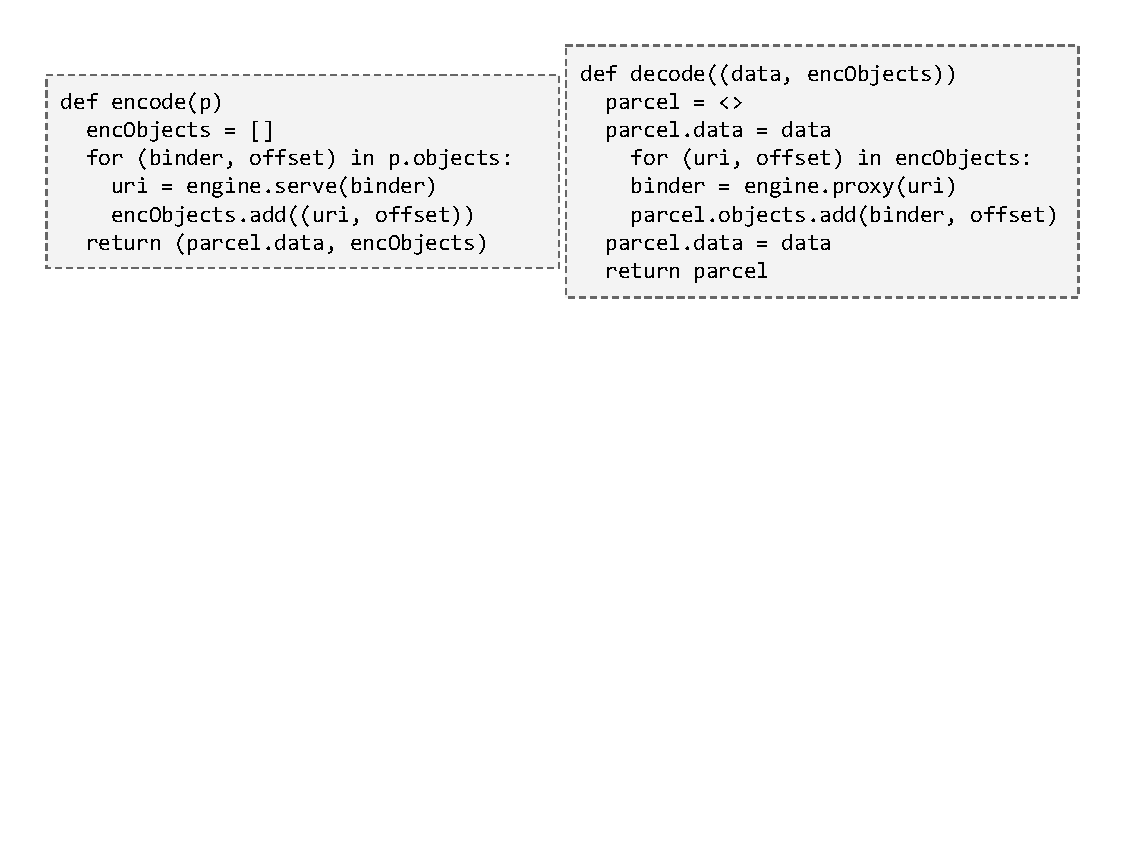
\includegraphics[width=0.8\textwidth]{drawings/encodeObjects.pdf}
\end{figure*}

Consider the example at the beginning of this section where getServiceManager() is invoked on the remote Sigma Engine. The reply Parcel contains a binder object. The remote Sigma Engine recognizes this and returns instead a URI to that object. On the client Sigma Engine, a new SigmaProxy object targeted to that URI is created while decoding the reply. The SigmaProxy is a special IBinder object that is returned to caller app on the local device. Invoking RPC on this IBinder creates a request over the network, invoking .transact() on remote ServiceManager.

\subsection{Dealing with parcels that contain file descriptors}

File descriptors in Parcels are handled analogously to binder objects. However, in Unix-like systems, file descriptors can refer to any Unix file type named in a file system. As well as regular files, this includes directories, block and character devices (also called "special files"), Unix domain sockets, and named pipes. File descriptors can also refer to other objects that do not normally exist in the file system, such as anonymous pipes and network sockets~\cite{UnixDomainSocket}.

Although it is theoretically possible to handle each type file descriptor (like the command-line utility nc that exposes each over a socket), each type of file descriptor has to be treated separately since each has a separate set of supported IO operations.

We only want to demonstrate as a proof-of-concept that we can handle file descriptors by focusing on a single type: the unix domain socket. These are used to communicate sensor events in SensorManager, and used elsewhere in GUI-related services. Such file descriptors are created via socketpair() with the protocol "SOCK\_SEQPACKET," providing sequenced, reliable, bidirectional, connection-mode transmission paths for records. A record can be sent using one or more output operations and received using one or more input operations, but a single operation never transfers part of more than one record~\cite{SocketManPage}. The only operations we are required to support are send() and recv(). Also the remote end needs to know when the socket is no longer valid or is otherwise closed so that resources can be cleaned up.

Encoding a parcel containing a file descriptor to a unix domain socket is much like encoding a parcel with binder objects. See the below pseudo-code. Unlike a service-oriented binder where request go only from client to server, the socket is bidirectional. Sigma Engines on both the local and remote device forward data and listen for incoming data on a thread.

\begin{figure*}
\centering
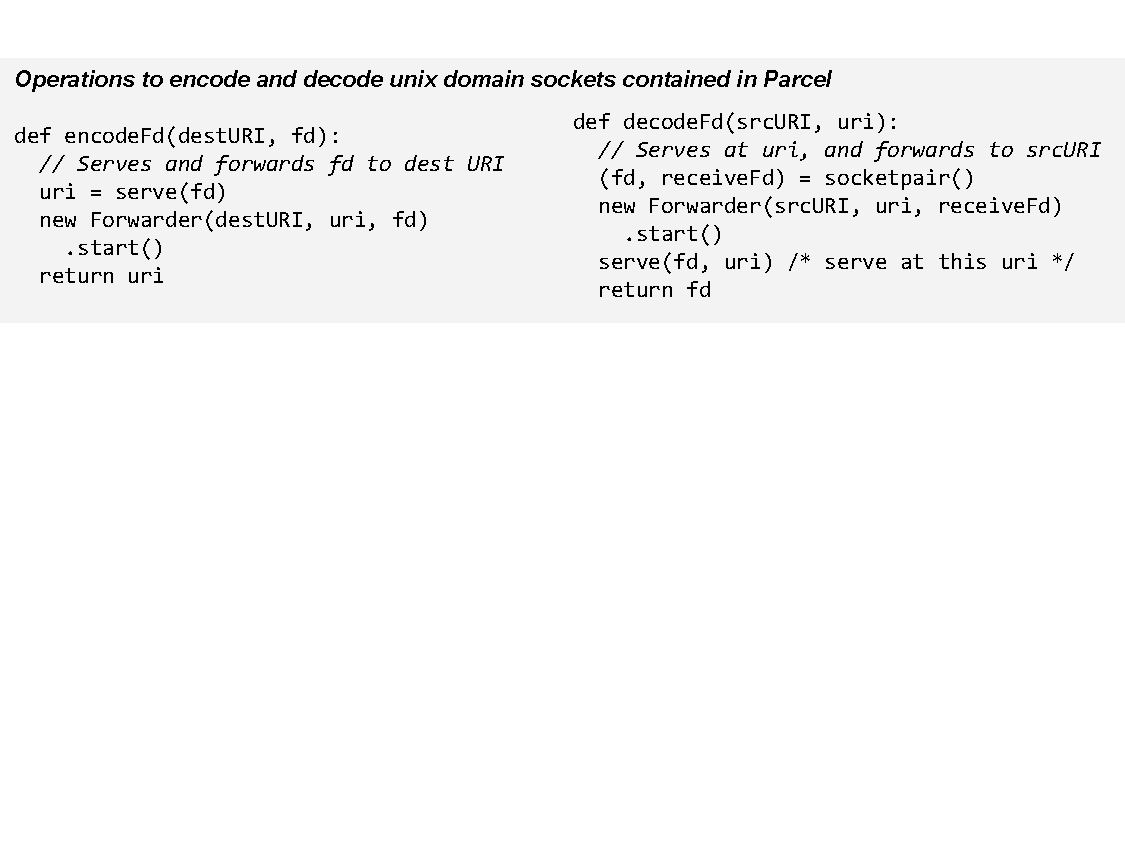
\includegraphics[width=0.8\textwidth]{drawings/encodeFds.pdf}
\end{figure*}

Creating and exchanging the URI for the file descriptor is only the first step. The Forwarder object then poll the file descriptor, locally received data is then forward over the network to addressed to the URI. Similarly, the remote device also sets up a forwarder so that data written to the socket from the remote-end will be received and forwarded locally. Data is received over the network is forwarded to the the duped file descriptor. Below is pseudo-code for the Forwarder thread on the client side, and events supported by the server. In the actual implementation, we use JNI to be able to poll() on file descriptors, as Java does not have any direct implementation.

\begin{figure*}
\centering
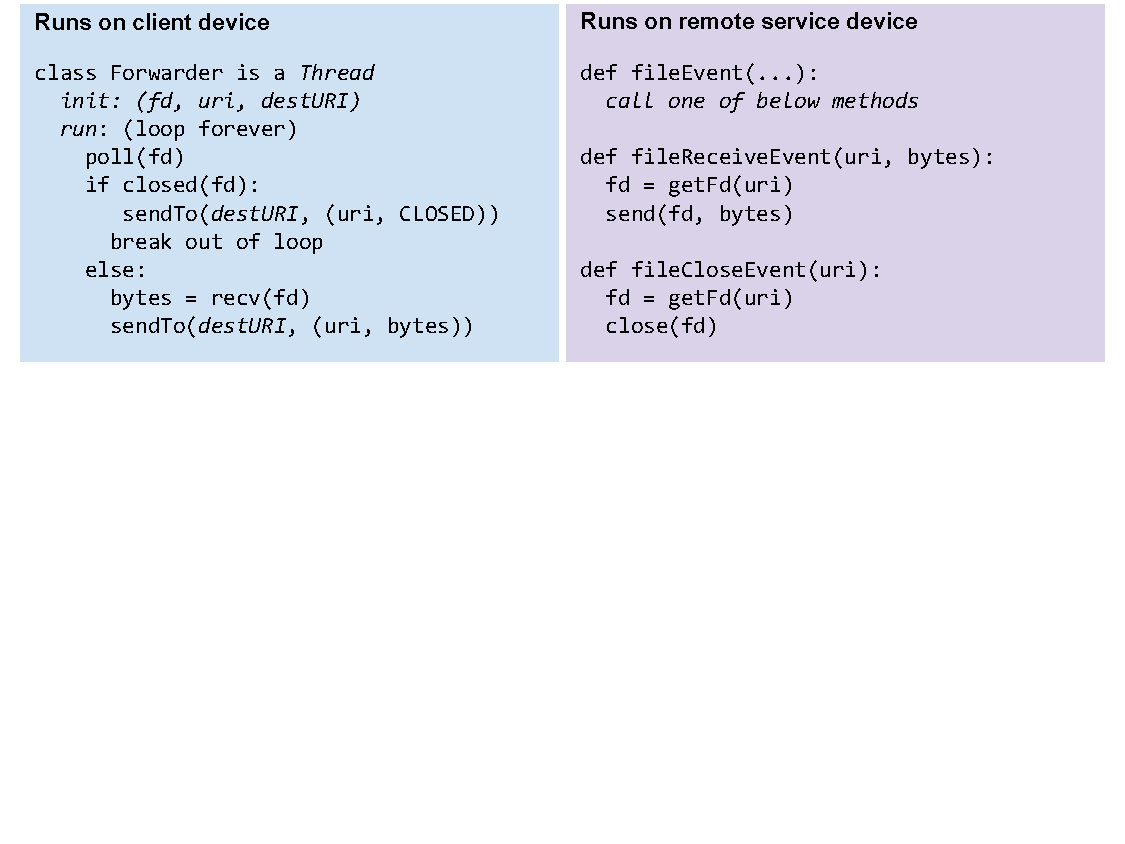
\includegraphics[width=0.8\textwidth]{drawings/forwardFds.pdf}
\end{figure*}

\subsection{Sigma Engine: Establishing a network data channel and subsequent communication}
Sigma first a protocol and then an implementation. As a protocol, it is agnostic to the network connection, assuming only that a reliable underlying connection channel is available for sending and receiving messages. For instance, one version of Sigma is implemented locally using Android Binder itself as a data channel. This is useful for testing as we can run two instances of Sigma engine on the same device. To evaluate Sigma between Android devices, we have a gamut of networking technologies to choose from. We choose HTTP- and XMPP- based channel to test evaluate the design and measure performance.

\subsubsection{Sigma Engine over HTTP}
In this mode, each device brings up a HTTP server listening on a pre-determined port. Clients communicate to another device by performing an HTTP POST request to another device's HTTP server. The client needs to know the IP or hostname of the server and the server must be accessible over the network.

\subsubsection{Sigma Engine over XMPP}
In this mode, each device logins to a mutually accessible XMPP server. XMPP is a popular protocol for real-time collaboration--messaging and chat. Clients make use of the same login as the server, communicating to other devices via uniquely identified chat threads. Each thread serves one transaction, similar to what is available in one HTTP POST request. Chat threads are limited to one request and to one reply. Future (or parallel) transactions occur on separate threads.

\subsubsection{Wire messages over the network}
The Sigma Engine creates Wire messages for each transaction. These can be printed to human-readable format. For instance, here is a URI to an XMPP-based SigmaEngine.

\begin{Verbatim}[samepage=true]
URI{_interface=com.example.BinderSigma.samples.chat.ICommentReceiver, domain=quark, login=rr, protocol=XMPP, type=BINDER, uuid=c2f980b5-ae50-4f7e-9559-438abc49508f}
\end{Verbatim}

Such Wire messages are compactly serialized into byte arrays. Over HTTP, the byte array is sent directly via a POST request as a byte-array entity. Over XMPP, the byte array is first made into a Base64-encoded string and then sent as a chat message. Below is an example of a SRequest sent as an XMPP chat message (note: the SRequest is serialized then Base64-encoded)

\begin{Verbatim}[samepage=true]
<message type="chat" id="30e5a4c7-b0d7-4d11-bd2c-14abf4ff1ce0"
        to="kk@quark" from="rr@quark/Smack" >
        <body> <!-- Base-64 encoded string --> </body>
        <thread>877a1f <!-- id of transaction --> </thread>
        </message>
\end{Verbatim}

The following set of figures show in detail the Wire messages exchanged between two Sigma Engines (implemented via a LOCAL protocol, with engines running on same device and communicating to each other via native binder). The messages correspond to the example from the beginning of "Design of Sigma" section, where a remote Sigma Engine reference is first retrieved via RPC to a local Sigma Engine, and then a reference to remote service is obtained.

Here, since we are operating under the LOCAL protocol, all transactions proxy binder objects are transit through the local Sigma Engine and then to the remote Sigma Engine (which also runs on the same device as a different process), and then from there to the native binder service. Naturally this the transit from local to remote Sigma Engine will take over the network (through HTTP or XMPP) for those implementations.

An exchange of Wire messages detailing a recursive binder that take place between two Sigma Engine instances is provided in the Appendix

\subsection{Sigma Engine as a binder service}
Using Sigma Engine's proxy facility, we can implement a remarkably simple service interface that can be used by app developers to connect first to a remote SigmaManager and use it retrieve remote reference to remote binder services.

\begin{Verbatim}[samepage=true]
interface ISigmaManager {
    URI getBaseURI();
    ISigmaManager getRemoteManager(
      in URI targetBaseURI);
    IBinder getServiceManager();
    /* synchronous version of
       bindService(Intent...) */
    IBinder getService(in Intent intent);
}
\end{Verbatim}

A device first access its own local Sigma Engine instance as a binder service, and can invoke a the local .getRemoteManager() with a remote URI as reference to obtain a reference to a remote Sigma Engine, again as a binder service--this time it is remote proxy. So in this way, the various operations of Sigma itself are implemented using binder and the Sigma proxy facilities

\begin{figure*}[t!]
\centering
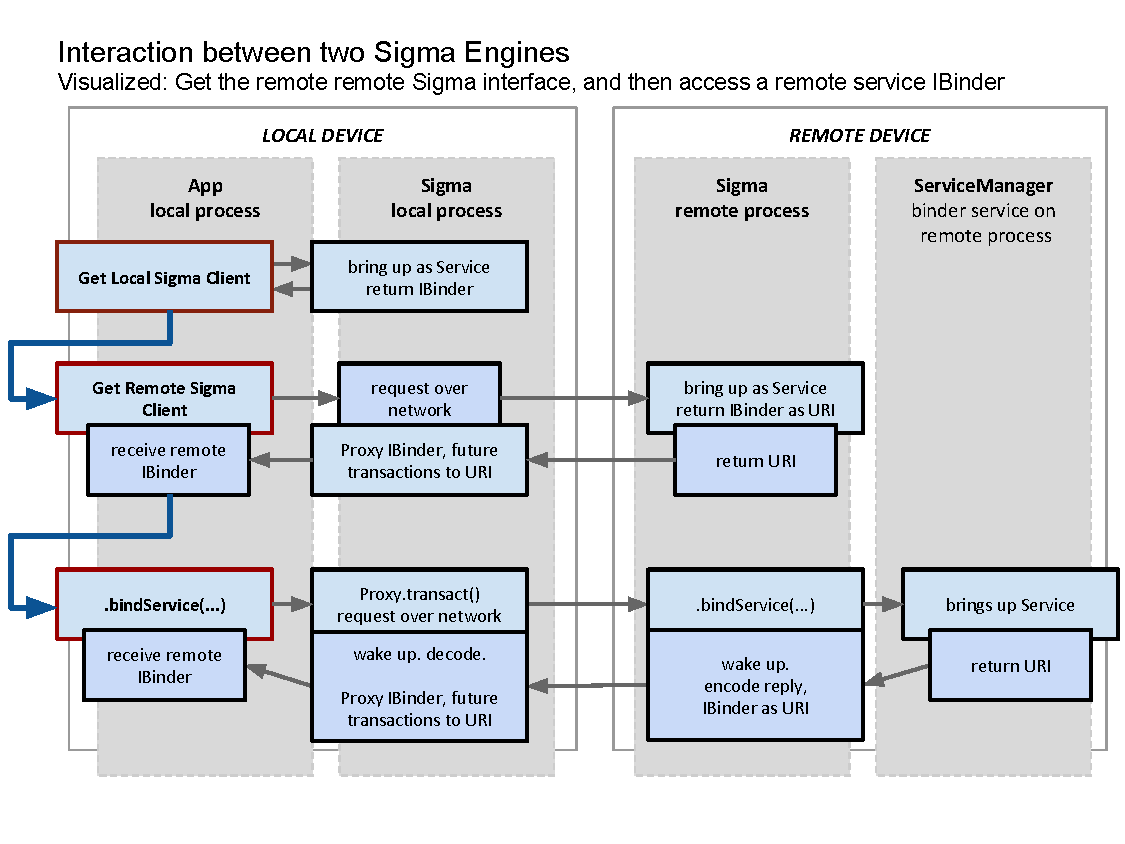
\includegraphics[width=0.8\textwidth]{drawings/SigmaEngineInteraction.pdf}
\end{figure*}

An app needs to know (through an initial exchange through a separately established channel) the URI for another Sigma-enabled device. And the app can obtain ISigmaManager service provided by the local Sigma Engine instance via a usual bindService() to get a local binder service. By calling localEngine.getRemoteManager(remoteURI), the app can obtain a reference to theISigmaManager service provided by the Sigma Engine on the remote device. The local Sigma Engine takes care to proxy RPCs to the remote Sigma Engine.

Besides the ability to obtain remote Sigma Engine instances, there are 2 other services provided by Sigma Engine: getServiceManager() and getService() that implement the two pathways to retrieve references to Android binder service. Invoking these RPCs on a Sigma Engine instance retrieves the requested service running on the same device as the engine. Having obtained a reference to a remote Sigma Engine, invoking these RPCs retrieves the remote binder services. A detailed example of this provided at the end of the next section.

\subsection{Performance: measuring CPU overhead and network latency}
It is useful to know the CPU cost and latency to establish a proxy to a remote binder service and then the cost to make Proxy RPCs. Overhead is expected due to the additional IPC within each device (there is communication from apps and services to the Sigma Engine). There is also the cost of encoding/decoding parcels during binder transactions, of creating requests and response messages, and naturally there is some cost to have network stack perform IO.

As a first test, consider a trivial binder service: a random number server. The interface is below.
\begin{Verbatim}[samepage=true]
class RandomServer extends IRandomServer.Stub() {
  int getRandom() { 
    return (new Random()).nextInt(); }
}
\end{Verbatim}


\begin{Verbatim}[samepage=true]
class PingPongService extends
    IPingPongService.Stub() {
  void ping(IPingPongService other, int count) {
    if (count > 0) other.pong(this, count - 1);
  }
  void pong(IPingPongService other, int count) {
    if (count > 0) other.ping(this, count - 1);
  }
}
\end{Verbatim}

As a second test, consider using binder to pass in binder objects as arguments. In particular, using this feature it is possible to specify a callback object that invokes a binder transactions back to the local device. Taking it one step further, recursion can occur back-and-forth as a series of binder calls between the two devices. The following binder service called PingPongService implements such a test. A local instance is passed in to invoke a method on the remote instance, like so: remote.ping(local, 10). This causes a cascade of recursive calls, each counting down the number argument.

Here is the result: the 3 types of calls from the preceding discussion are timed for various prototype implementations, and are described in the figure below.

\begin{figure*}
\centering
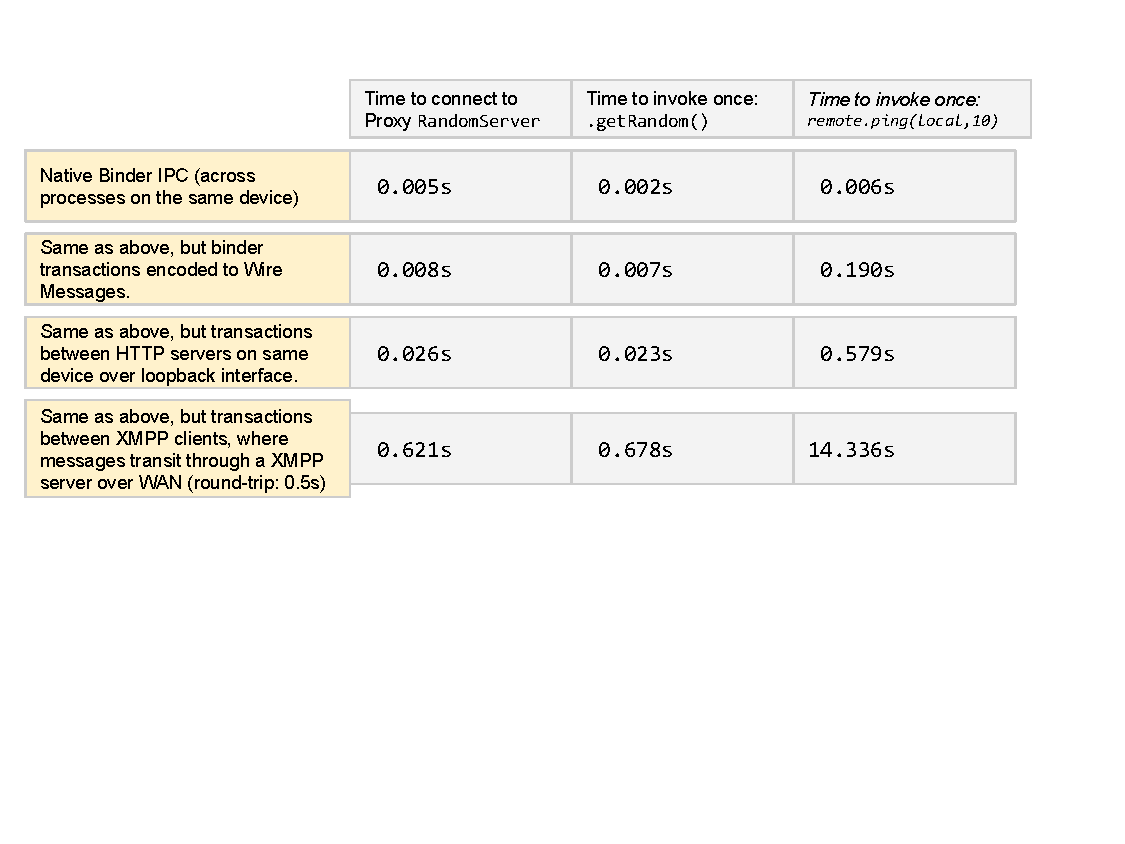
\includegraphics[width=0.7\textwidth]{drawings/Performance.pdf}
\end{figure*}

As is apparent, it is 2x-3x as expensive to perform a binder call over a proxy that encodes messages than it is to make a straight, native binder call. However, the recursive PingPong test is quite expensive since each recursive call is a new binder transaction with another round of encoding and decoding, with added network overhead.

\section{Example applications}

\subsection{Accessing remote system services}
All system services are published to the ServiceManager. However, the remote service interface is often not the final interface used by client apps. Often the remote interface is wrapped up in another local client object that provides the service to clients. Each app has an associated local runtime Context which provides clients a getSystemService(name) method that retrieves a remote system service as a binder object and then constructs a local client object for that service. Thus the remote service interface is usually hidden in the SDK, but available through reflection as the classes exist on any Android device or emulator.

Sigma provides a convenient RemoteContext class that is constructed with reference to a remote ServiceManager. It provides a mirror getSystemService(name) method that implements code to retrieve binder service (remote to another device, in this case) and constructs a local client object with reference to that remote service. Each system service needs some local code to wrap remote interfaces. As a proof-of-concept we have implemented the retrieval of two remote service--the LocationManager and SensorManager.

The following assumes knowledge of the respective system services, a overview of which is provided at the beginning sections of the paper.

\subsubsection{LocationManager}
We demonstrate that location updates can be requested from a remote device. As we have already demonstrated that binder object callbacks are supported by Sigma (see the above PingPong example), in this test we request location updates with the PendingIntent approach.

We have implemented the demonstration with location updates streamed from a real device (a Nexus 4) to an emulator running on a PC. The data channel is an XMPP-based channel, with a central XMPPl server located on the internet (in Amazon EC2, with a round-trip time from the device to the cloud is ~500ms). Both devices login as separate handles into this XMPP server.
Below is a diagram detailing the binder objects shared with between the Nexus 4 and emulator.

\begin{figure*}
\centering
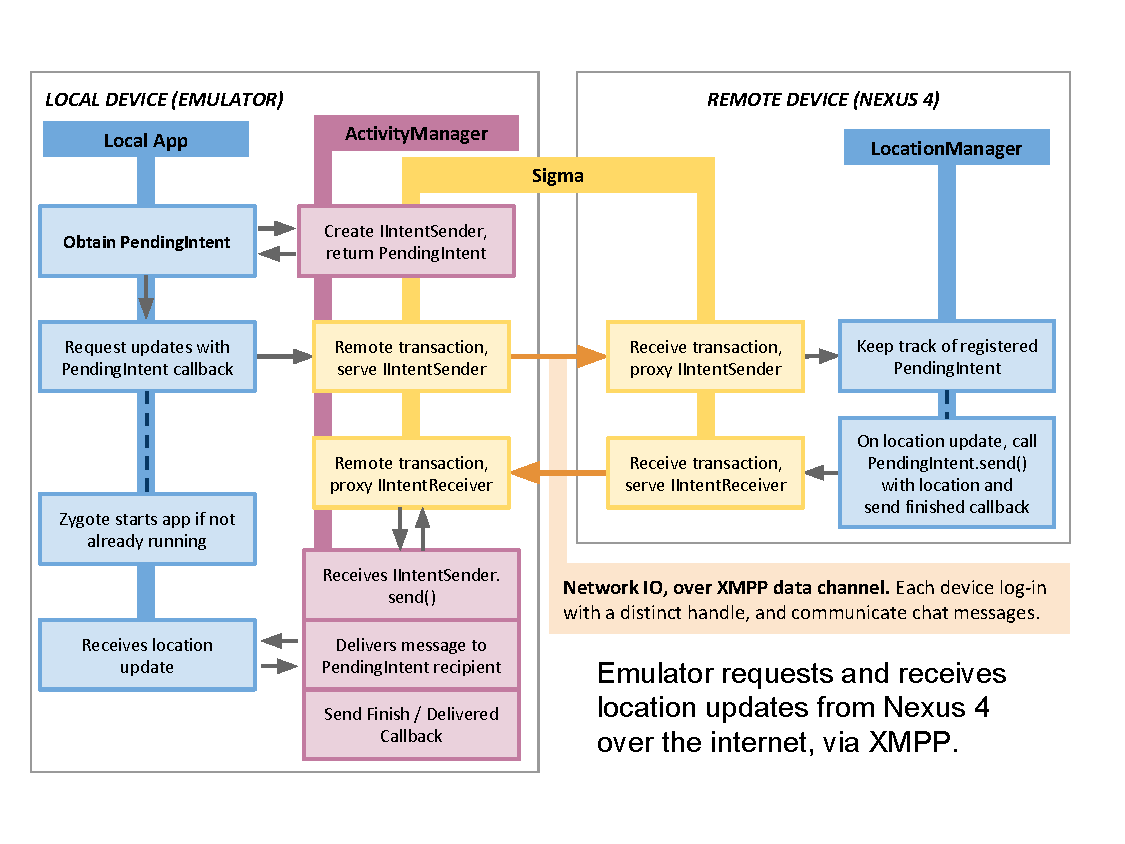
\includegraphics[width=\textwidth]{drawings/LocationPendingIntentExample.pdf}
\end{figure*}

Useful metrics to measure include CPU load, memory usage, and network utilization on participating devices. Memory usage includes tracking heap allocation over time and also to track the number of native binder objects held by each device. 

\subsubsection{SensorManager}
The request to register for sensor events creates a SensorEventConnection which contains a BitTube object that is essentially an OO version of unix domain sockets, with file descriptors communicated via binder. Subsequent communication happens via the socket. We demonstrate that socket events are proxied and forwarded by Sigma. And plot the time difference between the native sensorevent callback and the remotely-routed sensor callback. Of course, the data channel used will have an impact on delay, and so we plot three different versions, each with progressively more latency and jitter

\begin{figure*}
\centering
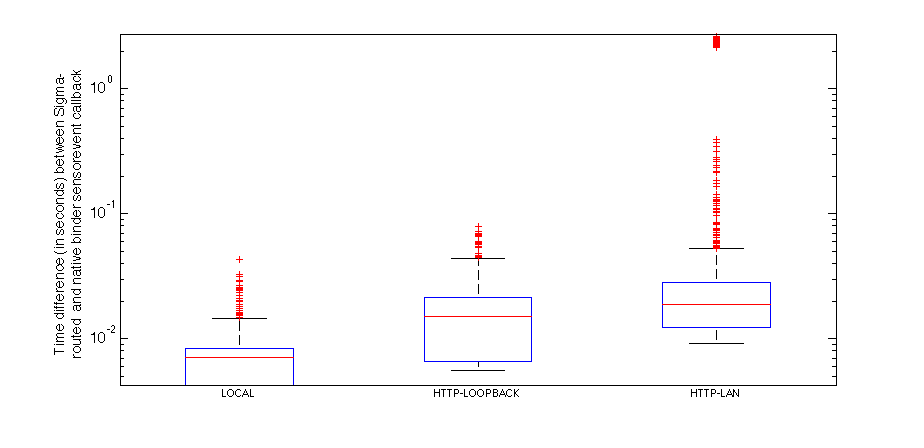
\includegraphics[width=\textwidth]{plots/sensorevent_delay.png}
\end{figure*}

Because there is jitter in received sensor events, it is necessary to depend on the timestamp provided by the sensorevent and not the timestamp of when the event is received by the listener callback. Also, depending on network conditions, it may not be possible to send sensor events at the full rate. Since Sigma is implemented with the assumption of a reliable, ordered underlying data channel: limited bandwidth results in progressively increasing latency. Below we have simulated a limited bandwidth situation by enforcing a delay on HTTP packets on LAN. After increasing latency we see that packets are dropped (or have not made it yet over the network) and the latency stabilizes to some large amount.

\begin{figure*}
\centering
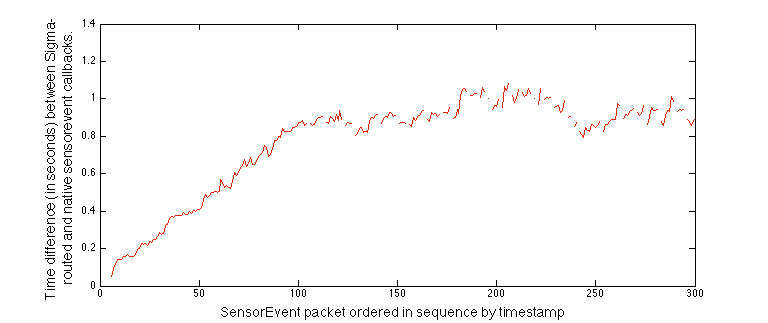
\includegraphics[width=\textwidth]{plots/limited_bandwidth_increasing_latency.png}
\end{figure*}

\subsection{Design of a Picture Sharing Service}
\begin{figure*}
\centering
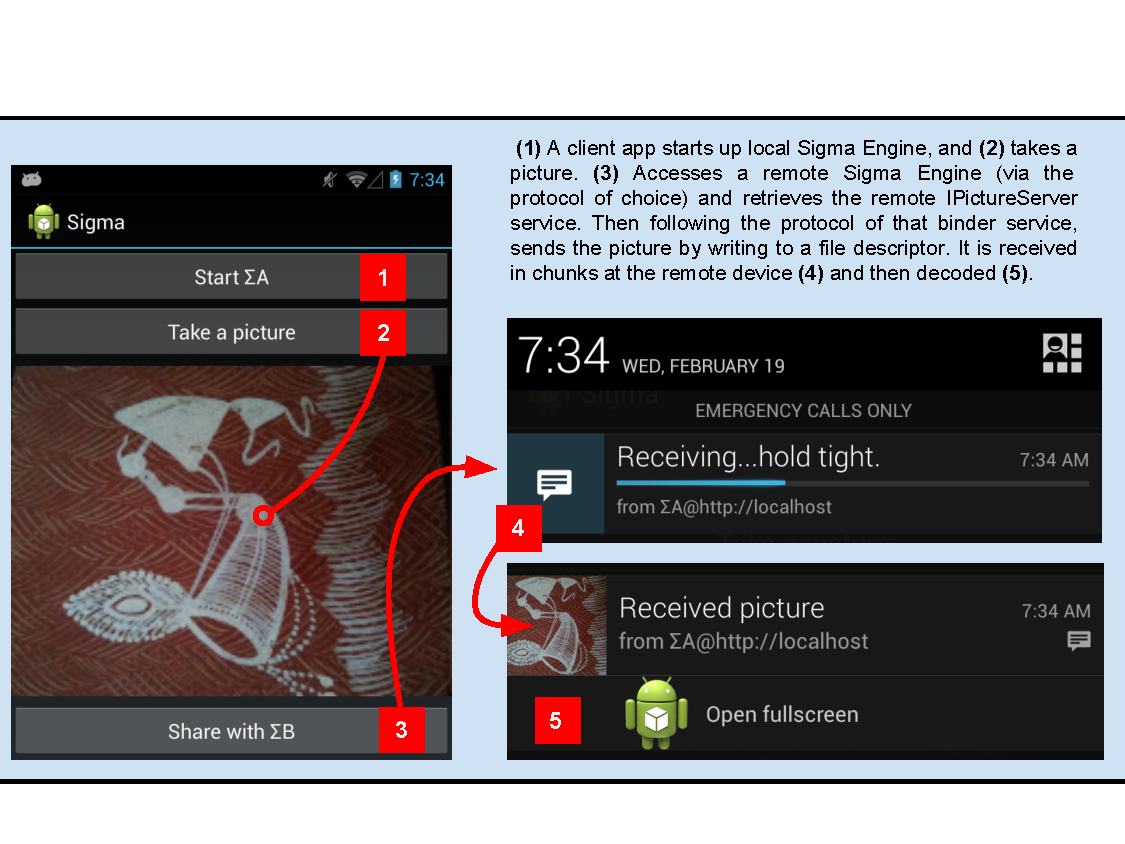
\includegraphics[width=\textwidth]{drawings/PictureChatExample.pdf}
\end{figure*}

\begin{Verbatim}[samepage=true]
interface IPictureChatServer {
  // Returns a fileDescriptor to which caller writes picture data.
  // Server polls the fileDescriptor to locally receives picture.
  // Sigma takes care of proxying file descriptor over network.
  // Also returns (modifies) PictureEntry with metadata as a new id for picture
  // used for subsequent request to the server.
  ParcelFileDescriptor /* readFrom */ requestPicturePut(
    ISigmaManager caller, inout PictureEntry entry);

  // Client passes in fileDescriptor to which server will write picture data.
  PictureEntry requestPictureGet(
    ISigmaManager caller, String uuid, in ParcelFileDescriptor writeTo);
}

class PictureEntry implements Parcelable {
    String uuid, from;
    int numBytes;
}
\end{Verbatim}


The design involves a single Binder service that acts as a picture server. Clients connects to remote picture server to upload (or share) a picture. The service interface could have been one that receives the picture as single large byte array. However, to make the implementation more interesting as a test, the PictureChatServer operates on put- and get- requests which operate on returned or passed-in file descriptors, respectively. Picture data is communicated from one end to the other by performing IO on these file descriptors

The PictureChatServer already (via native bidner) allows remote processes to connect to it to put or get pictures. With Sigma an app on a remote device can access the same PictureChatServer service. Thus, a picture sharing app can be implemented simply by writing a regular Android binder service and add make it into a distributed app with Sigma.

By requiring caller Sigma Engine to be passed itself in as an argument (i.e. the "ISigmaManager caller" argument), the PictureChatServer can invoke RPCs to get details about the caller device and credentials. Here in this example, we use it to get the name and protocol of the remote caller. In the future, we expect this is useful to authenticate and restrict callers.


\section{Discussion and next steps}
Sigma is not a finished product, nor is it the ultimate distributed communication mechanism. Rather it is a good starting point for experimentation with Binder as a distributed communication mechanism. There are still some deficiencies that need to be fixed up, and important features of Binder remain unimplemented.

\subsubsection{Sigma as it is implemented today is not compatible with vanilla Android}
We have implemented Sigma as an Android APK that can be installed on all devices. Much of the internal Java Android Runtime is hidden in the SDK, but is accessible by to applications by employing reflection. Much of Sigma is implemented this way. For instance, here's how we retrieve the internal ServiceManager from Java.

\begin{Verbatim}[samepage=true]
IBinder binder = sigma.getServiceManager(remoteURI);
Object serviceManager = Class.forName("android.os.ServiceManagerNative")
                    .getMethod("asInterface", IBinder.class)
                    .invoke(null, binder);
\end{Verbatim}

However, some of the objects needed are encapsulated and not accessible from Java without the appropriate implementations in JNI to expose native objects. Without resorting to extreme hacks (like poking into memory addresses~\cite{FacebookDalvikHacks}) we cannot run Sigma on a vanilla Android device. We need to make some minor modifications first. These were detailed in the previous section.

\subsubsection{System services not portable across Android versions}
The remote procedure call interface for system services is generated by the AIDL compiler. The generated remote procedure call interface can change with the changes to AIDL source and with different versions of the AIDL compiler. For instance, a method foo() may be assigned code=1 in one version, and code=2 in another. Naturally, when calling the same remote procedure interface across devices, a device can only know and operate on its own version of the generated interface.

The above limitation does not apply to services generated by other developers in the development of third-party apps using Sigma, as long as it is ensured that the same generated RPC interface is used between two devices. Unfortunately, generated AIDL interfaces do not have a notion of "versions" and it is impossible to tell from the Binder level whether two implementations of an interface (that go by the same) share the same generated structure.

\subsubsection{Parcels not portable between architectures}
Parcels were not made portable (over the network) and do not support sending marshalled packets over the network. One stumbling block is that fact that parcels can have objects in them like descriptors for local binders and file descriptors, and these are meaningless when ported to another system. That's why we went through all the trouble to serving each such objects over the network and create a proxy for each on the remote device.

There is still one aspect of parcels that is non-portable, and this since we copy the primitive data in the parcel's byte array byte-for-byte, it happens preserves endianness. This fact is troublesome since a remote device of the the opposite endianness would incorrectly process primitive data elements when it comes time to read each element out of the parcel.
Although this is a seemingly major obstacle to the use of binder as a distributed communication mechanism, in practice we see that most all Android devices are ARM-based, and ARM chips are bi-endian (there is a little switch to toggle to specify the endianness). Android, by specification, is little-endian for all such ARM-based devices~\cite{ARMLittleEndian}.

There is a way to make parcels portable, but we leave that as future work. The basic deficiency is that Parcels do not store about what was written into them where (i.e. the offset into the data array and size of the element written). There is no such metadata available in-band inside the parcel's data array or out-of-band in the other member variables of the parcel object. To allow for portability, we would need to interpret each element written into data array (is it an integer or a string of some length or something else?). Or we need to know the offset of each element and its size in the array. The idea then is to marshall each object separately using a canonical choice for its endianness (see how protobufs deal with endianness). Unmarshalling back into the data array would need to follow an analogous reverse procedure reading each object in the marshalled parcel and storing it in the appropriate native endianness of the system. Essentially the Parcel would need to store additional metadata about its contents.

\subsubsection{XMPP and HTTP are not entirely satisfactory as data channels}
HTTP is only suitable over the local network since a HTTP server running on a device behind NAT is not accessible by others without additional configuration. XMPP uses a central chat server (accessible to all other devices) as a middleman. Having such a middleman incurs a performance penalty, and possible privacy concerns.

There are new technologies such as WebRTC that seek to establish fully peer-to-peer connections. A signalling channel such as XMPP is used first to exchange descriptors between devices, and then a central server (typically hosted publically by a third-party) is involved in establishing a direct peer-to-peer connection. All subsequent communication is done via this connection. This same technology is used by Google Talk, and is soon going to become a w3c standard. Implementing and evaluating binder over network using webrtc data channels is left for future work.

\subsubsection{Availability}
What happens when connection is lost if the remote binder object is not available? The local binder supports registering a "linkToDeath()"  callback which invokes the binderDied method of the callback when the host service process dies. This is fortunate because using this mechanism we can also have such notifications over the network. However, this feature is not currently implemented in the prototype.

Another feature of Android Binder (not the BKM) is that a RemoteException is thrown when binder RPC throws an exception on the remote side. Parcel objects (and the auto-generated RPC interface) support the writing of exceptions as the reply, and are read on the local proxy side. These exceptions are supported automatically. 

\subsubsection{Binder over network breaks Android security model}
Each Android app has an a belongs to a java package namespace. The PackageManager keeps track of the set of permissions that are requested by the package and also holds a map of the user-id assigned to each active package. Android activities and services within a package run as one or more processes which share the same user-id.

System services typically run as the root user. When an app (the caller) uses Binder IPC to make a call to another process like a system service, the callee can look up the process-id and user-id of the caller. This facility is baked into the BKM which is the component that handles the context switch from the caller to the callee (i.e. the caller thread sleeps, and wakes up a receiving thread in the callee's process). The callee can figure out (with the help of PackageManager) whether the caller has permission to access that particular system service. The system service in this way can reject unauthorized calls. This is a runtime security feature provided by BKM.

When the caller happens to be a process on a remote device, the Android security model breaks down. As implemented now, binder services are accessed and bound to the Sigma Engine, and not the process on the local device. The latter option does not make sense anyway since the remote ActivityManager does not know about the local process. Right now, Android permissions are effectively circumvented by having the Sigma Engine declaring all permissions--i.e. it essentially runs with root permissions. Any security is implemented separately by the Sigma Engine. And the permissions declared by the local process do not come into play.

There are obvious concerns with running with full permissions. One idea would be the remote device to communicate with the PackageManager on the local device, and grant an app all the permissions it is granted on the local device. However, this solution does not seem entirely satisfactory. Imagine an application requesting permission to access location of the local (its own) device means that it can also access location on all other remote devices.

It makes more sense for an app to be given permission to use a set of local services, and then a separate set of permissions granted to use remote services. For instance, a configuration panel on the remote device, much like a firewall, can be used to allow other devices access to certain services. Whenever the PackageManager is tasked with checking permissions for a binder object owned by Sigma Engine, such requests are redirected to Sigma. The implementation of such a panel and the necessary modifications to PackageManager is left for future work.

\subsection{Next Steps}
In the long-term, it would be interesting to tightly coupling two connected devices within Android Runtime. Imagine that the local and remote PackageManager merge (in a decentralized way) and present each device's components in their own namespace--one local, the other remote. Permissions would have to be specified with the idea of a local and remote namespace as well. Consider also that the ActivityManager is merged. Sigma Engine would run within the runtime as part of the ActivityManager rather than as a separate package. With such tight coupling established, local components are able to connect to remote components directly through the ActivityManager's bindService(), specifying a "remote" or "local" namespace. Tight coupling also solves some issues with notifications of binder service death. Lifecycle events of Android components on one device would automatically notify the other device, etc.

\section{Appendix}

\begin{Verbatim}[samepage=true]
class IServiceManager : public IInterface {
 public:
    // Retrieve an existing service, blocking for a few seconds if it doesn't yet exist.
  virtual sp<IBinder> getService(const String16& name) const = 0;
    // Retrieve an existing service, non-blocking.
  virtual sp<IBinder> checkService(const String16& name) const = 0;
    // Register a service.
  virtual status_t addService(const String16& name, const sp<IBinder>& service, ..) = 0;
    // Return list of all existing services.
  virtual Vector<String16> listServices() = 0;
}
\end{Verbatim}


\begin{Verbatim}[samepage=true]
binder_call(binder_state *bs, binder_io *msg, binder_io *reply, void *target, int code)

bs- each binder transaction and service gets its own state. Essentially contains a file descriptor obtained via open("/dev/binder") which is used to communicate with the binder kernel module.
msg- essentially contains a data array with the following:
  * "android.os.IServiceManager" - name of the interface published in target binder service.
  * "com.example.service"        - name of the service to be  published
  * binder_service               - reference to the local binder binder; the service published
reply- contains the returned data array after the transaction. Can be null if there is no return value or we don't care about it.
target- is a reference to a remote binder service already published. Usually references are obtained by a binder_call to the ServiceManager to retrieve published services. However, we can always make a binder call to the ServiceManager itself, which is always at the address (void*)0.
code- is a non-specific value passed to the handler of the remote binder object. In this case, we pass an integer representing the action to be performed, where SVC_MGR_ADD_SERVICE is an pre-defined int.
\end{Verbatim}

All operations of a binder\_service are implemented inside of a handler function; the function signature resembles that of binder\_call:
\begin{Verbatim}[samepage=true]
service_handler(binder_state *bs, binder_txn *txn,  binder_io *msg,  binder_io *reply)
bs  - The initiating transaction.
txn  - essentially contains code (from binder_call), the calling unix process id and unix user id.
msg  - The message from binder_call.
reply  - The return value should be written out here, if any
\end{Verbatim}

\begin{Verbatim}[samepage=true]
struct flat_binder_object {
  unsigned long type, flags  /* header */
  union {
    void *binder;    /* local object */
    signed long handle;  /* remote object */
  };
  void *cookie;     /* extra data */
};
\end{Verbatim}

\begin{Verbatim}[samepage=true]
struct binder_io {
  char *data;            /* start of data buffer */
  uint32_t *offs;        /* array of offsets */
  uint32_t data_avail;   /* bytes available in data buffer */
  uint32_t offs_avail;   /* entries available in offsets array */
};
\end{Verbatim}

\begin{figure*}[t!]
\centering
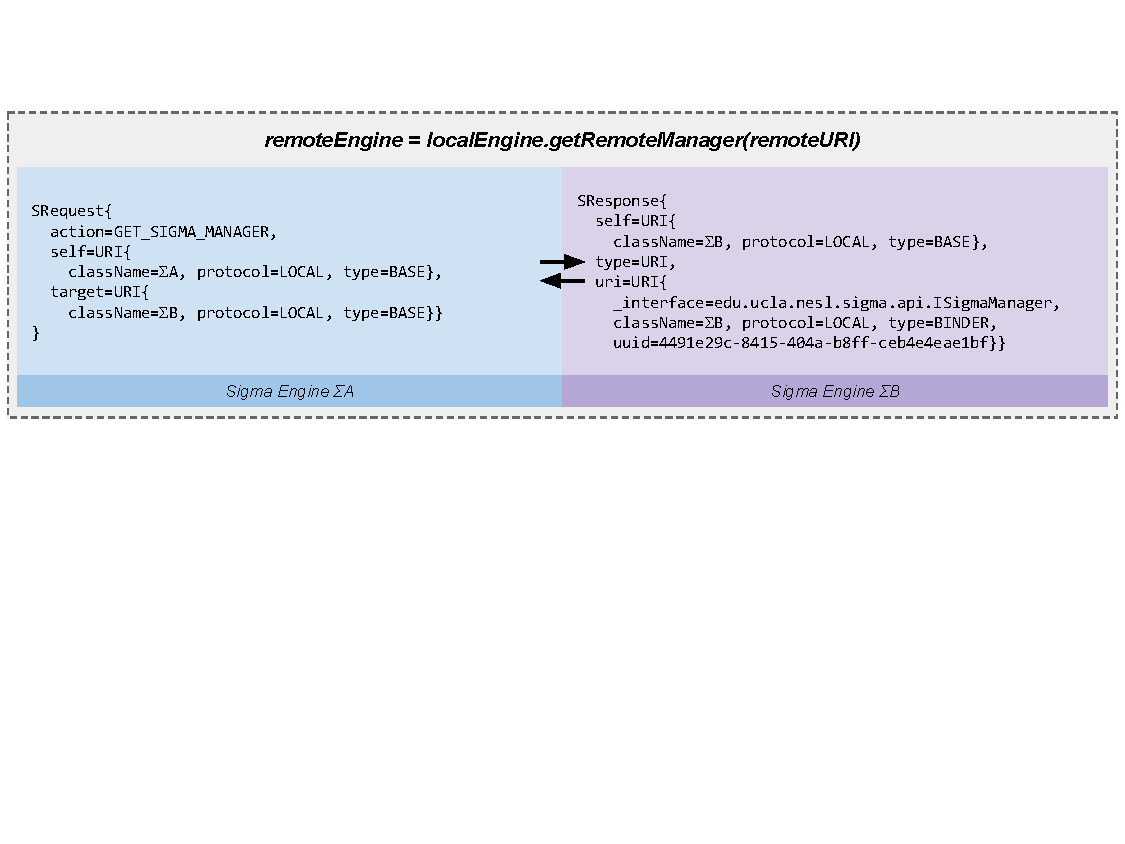
\includegraphics[width=\textwidth]{drawings/WireExchange1.pdf}
\end{figure*}


\begin{figure*}[t!]
\centering
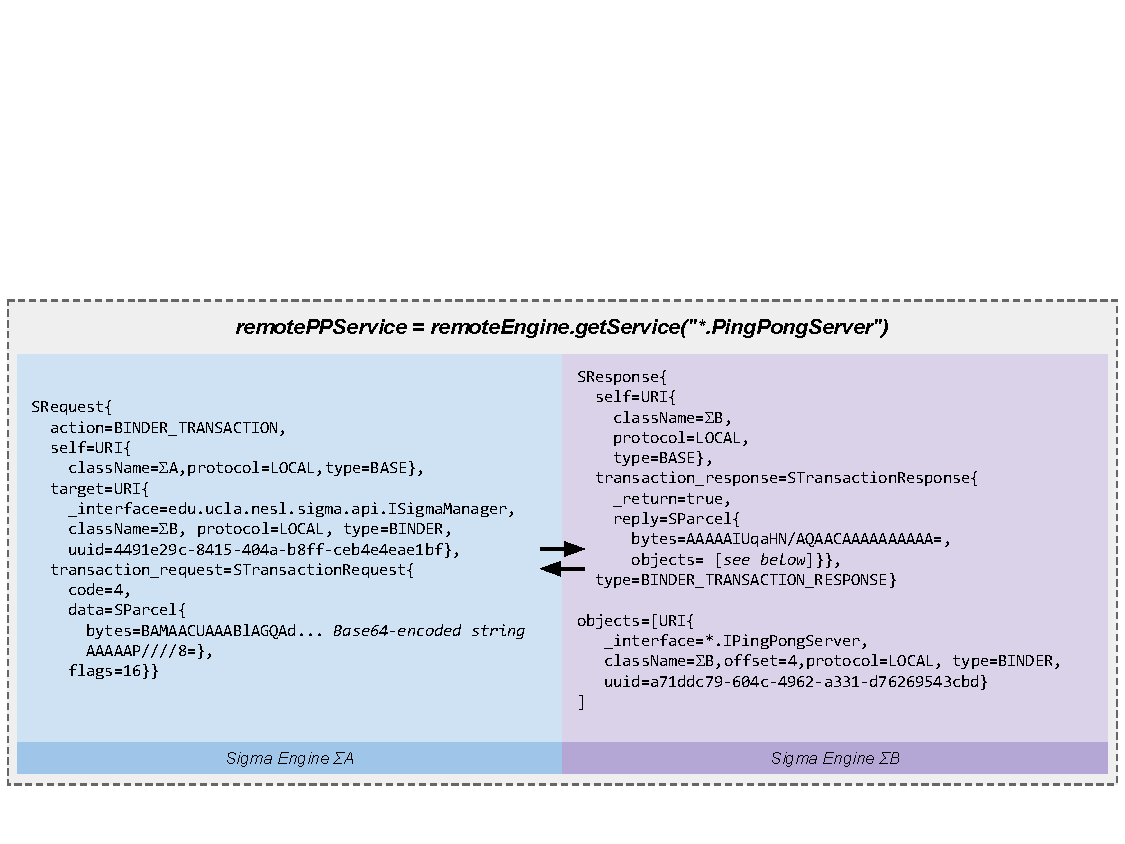
\includegraphics[width=\textwidth]{drawings/WireExchange2.pdf}
\end{figure*}


\bibliography{sigma}
\end{document}

